\documentclass{article}

\usepackage[margin=1in]{geometry}
\usepackage{amsmath}
\usepackage{amsfonts}
\usepackage{mathtools}
\usepackage{indentfirst}
\usepackage{bbm}
\usepackage{graphicx}
\usepackage{float}
\usepackage{tikz-cd}
\graphicspath{ {figures/} }

\title{Calibrating Perplexity in the Presence of Noise}
\date{}

\begin{document}

\maketitle

\section{Abstract}
The goal of dimension reduction tools is to construct a low-dimensional representation of a high-dimensional dataset. These tools are employed for a variety of reasons such as noise reduction, visualization, and to lower computational costs. However, there is a fundamental issue that is highly discussed in other modeling problems, but almost entirely ignored by the dimension reduction literature: overfitting. If we interpret data as a combination of signal and noise, dimension reduction techniques are judged only on how well they capture the original data (\cite{perplexity vs kl}, \cite{quantitative survey}, \cite{t-SNE cell}, \cite{rank-based criteria}, \cite{precision score}), i.e. both the signal and the noise. In the context of other modeling problems, techniques such as feature-selection, cross-validation, or regularization are taken to combat overfitting, but no such precautions are taken when performing dimension reduction. In this paper, we present a framework that models dimension reduction in the presence of noise. We then use this framework to explore the role perplexity plays in overfitting the data when applying t-SNE in order to demonstrate the importance of interpreting high-dimensional data as a combination of signal and noise. More specifically, we hypothesize t-SNE tends to overfit the noise when the perplexity is too low.

\section{Introduction}

\subsection{t-SNE}
The t-SNE algorithm captures the topological structure of the high-dimensional data by calculating directional similarities via a Gaussian kernel. The similarity of point $x_j$ to point $x_i$ is defined by $$p_{j|i} = \frac{\exp(-||x_i - x_j||^2/2\sigma_i^2)}{\sum_{k \neq i} \exp(-||x_i-x_k||^2/2\sigma_i^2)}.$$ Thus for each point $x_i$, we have a a probability distribution $P_i$ that quantifies the similarity of every other point to $x_i$. The variance of the Gaussian kernel $\sigma_i^2$ is chosen so that the perplexity, in the information theory sense, of the probability distribution $P_i$ is equal to a pre-specified value named perplexity, $$\textrm{perplexity} = 2^{-\sum_{j \neq i} p_{j|i}\log_2 p_{j|i}.}$$ Intuitively, perplexity controls how large a neighborhood to consider around each point when approximating the topological structure of the data. As such, it implicitly balances attention between local and global aspects of the data with high values of perplexity placing more emphasis on global aspects. For the sake of computation convenience, t-SNE assumes the directional similarities are symmetric by defining $$p_{ij} = \frac{p_{i|j} + p_{j|i}}{2n}.$$ The $p_{ij}$ define a probability distribution $P$ on the set of pairs $(i,j)$ that represents the topological structure of the data.

\bigbreak The goal is to then find an arrangement of low-dimensional points $y_1, \hdots, y_n$ whose similarities $q_{ij}$ best match the $p_{ij}$ in terms of Kullback-Leibler divergence, $$D_{KL}(P || Q) = \sum_{i,j} p_{ij} \log \frac{p_{ij}}{q_{ij}}.$$ The low-dimensional similarities $q_{ij}$ are defined using the t-distribution with one degree of freedom, $$q_{ij} = \frac{(1 + ||y_i - y_j||^2)^{-1}}{ \sum_{k \neq l} (1 + ||y_k - y_l||^2)^{-1}}.$$

\bigbreak The two main downsides of t-SNE are its randomness and dependence on the chosen perplexity. The minimization of the loss function is done using gradient descent methods with incorporated randomness to avoid stagnating at local minima. As a result, the outputted representation will differ between runs of the algorithm. Therefore, the traditional t-SNE workflow often includes running the algorithm multiple times then choosing the most desirable representation. As for calibrating perplexity, there is no universal rule-of-thumb. The original authors suggested values between 5 and 50 \cite{t-SNE}, while recent works have suggested perplexity values as large as $n/100$ \cite{t-SNE cell} for larger datasets. When calibrating perplexity, common practices include both qualitative and quantitative metrics. If the output dimension is two or three, we can visualize the results and choose the perplexity whose results best capture the hypothesized structure. When working with supervised data, for example, we look for representations that cluster according to the class labels. This method, however, has some limitations. In the case of unsupervised dimension reduction, it's not always clear what features are desired. Moreover, this method does not work when the output dimension is greater than three. In these cases, we rely on quantitative metrics.

\section{Methods}

\subsection{The Framework}
Suppose the underlying signal of our data is captured by an $r$-dimensional data set $Y \in \mathbb{R}^{n \times r}$. In the context of dimension reduction, the underlying signal is often lower dimension than the original data. Let $p \geq r$ be the dimension of our original data set, and let $\textrm{Emb}:\mathbb{R}^r \to \mathbb{R}^p$ be the function that embeds the signal in data space. Define $Z = \textrm{Emb}(Y)$ to be the signal embedded in data space. We then assume the presence of random error. The original data can then be written as $$Z + \epsilon \textrm{ for } \epsilon \sim N_p(0, \Sigma).$$ The dimension reduction method $\varphi$ is applied to $Z + \epsilon$ to get the low-dimensional representation $X \in \mathbb{R}^{n \times q}$.

\begin{center}
\begin{tikzcd}[sep=large]
                                                                    & Z + \epsilon \arrow[rrd, "\varphi"] &                          &   &    \\
                                                                    & Z \arrow[u]                         & Y \arrow[l, "Emb", hook] & X &    \\
{} \arrow[rrrr, "\textrm{Dimension (high to low)}"', shift left=5] &                                     &                          &   & {}
\end{tikzcd}
\end{center}

\bigbreak Now suppose we have a reconstruction error function $f(D_1, D_2)$ that quantifies how well a data set $D_1$ is represented by another data set $D_2$. Prior works study $f(Z + \epsilon, X)$ to measure how well the constructed representation $X$ represents the original data $Z + \epsilon$. We argue it is more appropriate to compare $X$ against the underlying signal $Y$ instead by studying $f(Y, X)$.

\subsection{Reconstruction Error Functions}
Prior works in dimension reduction have suggested various quantitative metrics for measuring dimension reduction performance (\cite{t-SNE cell}, \cite{quantitative survey}, \cite{rank-based criteria}, \cite{trustworthiness}). In line with recent discussions of perplexity \cite{t-SNE cell}, we focus on two metrics --- one for measuring local performance and one for measuring global performance.

\bigbreak For local performance, we employ a nearest-neighbor type metric called trustworthiness \cite{trustworthiness}. Let $n$ be the sample size and $r(i,j)$ be the rank of point $j$ point among the $k$ nearest neighbors of the point $i$ in high dimension. Let $U_k(i)$ denote the set of points among the $k$ nearest neighbors of point $i$ in low dimension, but not high dimension. Then $$f_{trust}(D_1, D_2) = 1 - \frac{2}{nk(2n - 3k - 1)}\sum_{i=1}^n \sum_{j \in U_k(i)} \left[ r(i,j) - k \right].$$ For each point, we are measuring the degree of intrusion into its $k$-neighborhood. The quantity is then re-scaled, so that trustworthiness falls between 0 and 1 with higher values favorable. Note, trustworthiness is preferable to simply measuring the proportion of neighbors preserved because it's more robust to the choice of $k$. For very large values of $n$, we can get an estimate by only checking a random subsample of points $i_1, \hdots, i_m$. In this case, $$f_{trust}(D_1, D_2) \approx 1 - \frac{2}{mk(2n - 3k - 1)}\sum_{l=1}^m \sum_{j \in U_k(i_l)} \left[ r(i_l,j) - k \right].$$

\bigbreak For global performance, we employ Shepard goodness \cite{quantitative survey}. A Shepard diagram is a plot of inter-point distances in high dimension vs. inter-point distances in low dimension used to understand how distances are stretched and shrunk during dimension reduction. Shepard goodness is the Kendall correlation (a rank-based correlation) between high and low-dimensional inter-point distances, $$f_\textrm{Shep}(D_1, D_2) = \sigma_\textrm{Kendall}(||x_i - x_j||^2, ||\varphi(x_i) - \varphi(x_j)||^2).$$ Again for very large values of $n$, we can get an approximation by calculating the correlation between inter-point distances of a random subsample.

\subsection{Constructing Examples}
When conforming examples to our framework, three components need to be specifed: $Z + \epsilon$, $Y$, and $\textrm{Emb}()$. These elements describe the original data, the underlying signal, and the embedding of the signal in data space, respectively. When generating examples, it's natural to start with the underlying signal $Y$ then construct $Z + \epsilon$ by attaching extra dimensions and adding Gaussian noise. The $\textrm{Emb}()$ function is then given by $$\textrm{Emb}(y) = (y,0,\hdots,0),$$ so that
$$Z + \epsilon = \begin{bmatrix}
Y & \vert & 0
\end{bmatrix} + \epsilon.$$

\bigbreak Practical examples are more tricky because we do not have the luxury of first defining $Y$. Instead, we are given the data $Z + \epsilon$ from which we must extract $Y$, or at least an estimate. The best way to accomplish this is a topic for further exploration, but we opted for $Y = \textrm{PCA}_r(Z + \epsilon)$. For a reasonable $r$, we'd expect the first $r$ principal components to contain most of the signal while excluding the noise. Although $f(Y, X)$ is no longer an exact comparison to the signal, it is a reasonable estimate that's more faithful than $f(Z + \epsilon, X)$. Another advantage to using PCA is it gives rise to a natural $\textrm{Emb}()$ function --- the PCA inverse transform. This linear transform is readily available and quick to compute.

\section{Results}

\subsection{Generated Examples}

We first look at generated examples that exaggerate the affect of perplexity on the t-SNE output: inter-linked circles, the trefoil knot, and the mammoth dataset \cite{understanding DR}.

\begin{figure}[H]
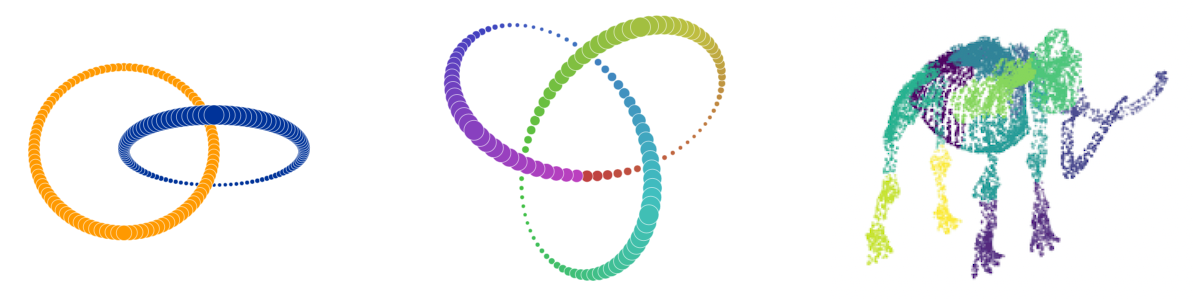
\includegraphics[scale=0.4]{links}
\centering
\caption{Generated Examples (Links and Trefoil from \cite{Distill}, Mammoth from \cite{understanding DR})}
\end{figure}

For each example, the signal $Y$ consisted of 500 points in three dimensions. The dataset $Z + \epsilon$ was constructed from $Y$ by first adding seven superfluous dimensions then adding isotropic Gaussian noise to all 10 dimensions. We then ran t-SNE using the $R$ package \textit{Rtsne} with perplexity values ranging from 10 to 160 (\textit{Rtsne} implements a Barnes-Hut approximation that only allows for a maximum perplexity of $\frac{n-1}{3}$). For each value of perplexity, the algorithm was ran 20 times to mimic the ordinary t-SNE workflow. If we were to disregard the distinction between signal and noise, a plot of $f_\textrm{Shep}(Z + \epsilon, X)$ vs. $f_\textrm{trust}(Z + \epsilon, X)$ could be used to calibrate perplexity. To avoid overfitting the noise, a plot of $f_\textrm{Shep}(Y, X)$ vs. $f_\textrm{trust}(Y, X)$ should be used instead. Below are the two plots for the links example:

\begin{figure}[H]
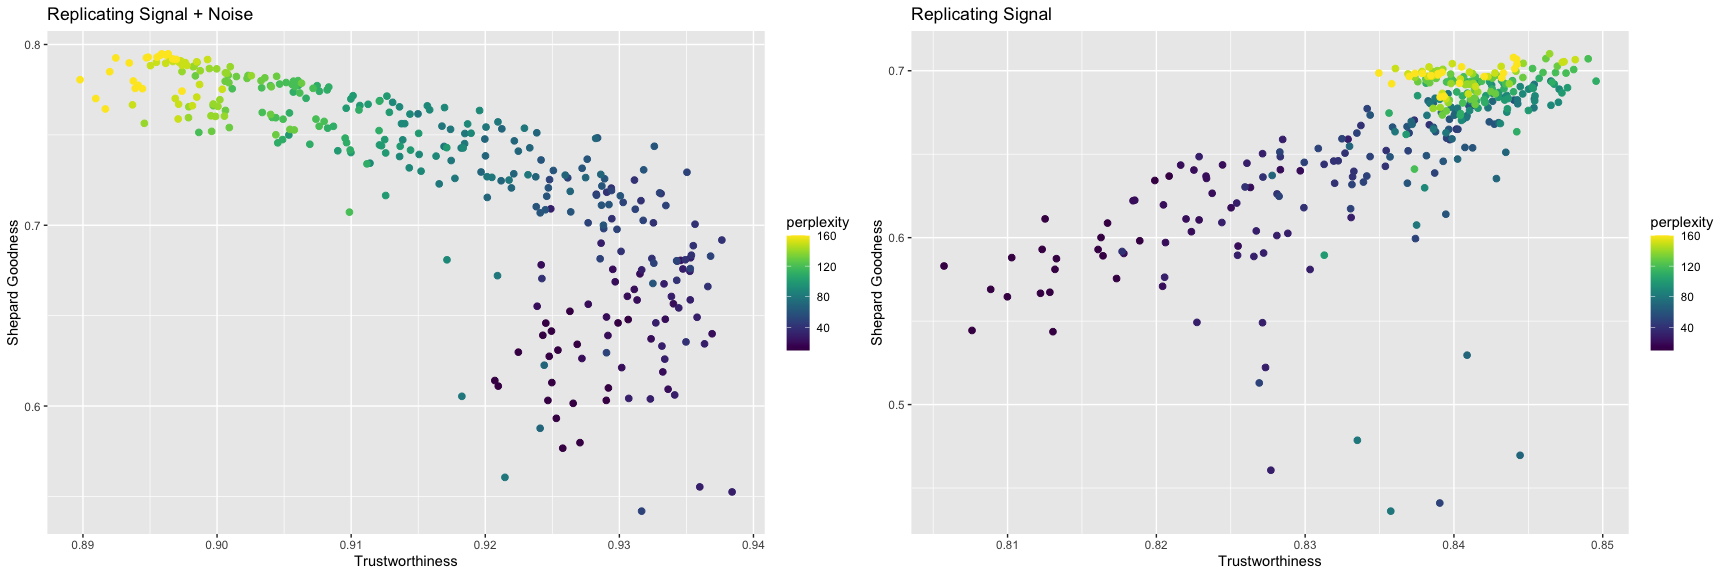
\includegraphics[scale=0.25]{links plot}
\centering
\caption{Shepard Goodness vs. Trustworthiness (Links)}
\end{figure}

Both plots depict an increase in global performance as perplexity increases. In terms of local performance, both plots show an increase in perplexity followed by a decreases as perplexity increases. This is more evident when we plot trustworthiness vs. perplexity:

\begin{figure}[H]
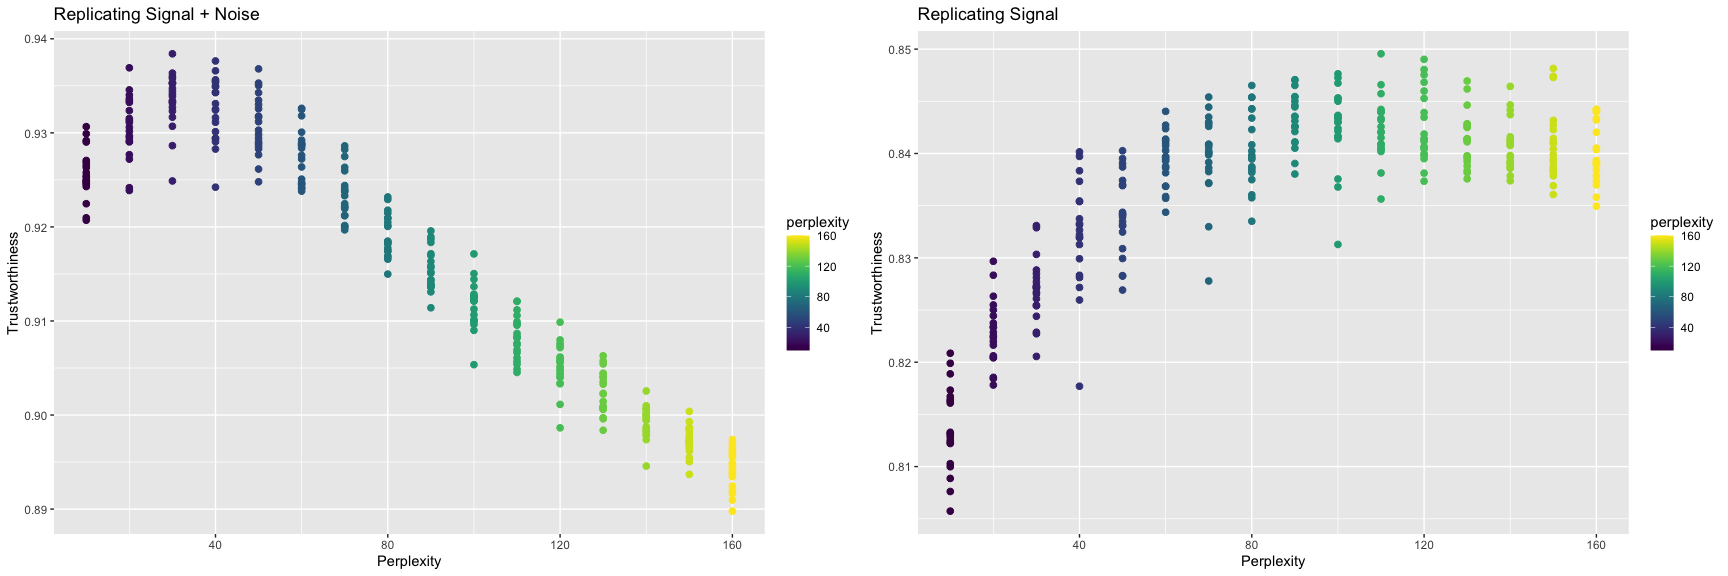
\includegraphics[scale=0.25]{trust plot (links)}
\centering
\caption{Trustworthiness vs. Perplexity (Links)}
\end{figure}

Past a certain perplexity, local performance deteriorates as a perplexity increases, exhibiting the trade-off between global and local performance. This cutoff point, however, varies between the two plots. When comparing against the original data, a perplexity of slightly below 40 seems to maximize trustworthiness. This is consistent with the original authors' suggestion of 5 to 50 for perplexity \cite{t-SNE}. When comparing against the underlying signal, a perplexity of around 120 maximizes trustworthiness. From this phenomenon, we hypothesize t-SNE tends to overfit the noise when the perplexity is too low. Intuitively, small perplexities are more affected by slight perturbations of the data when only considering small neighborhoods around each point. Conversely, larger perplexities lead to more stable representations in the presence of noise.

\bigbreak The other two generated examples exhibit the same trend:

\begin{figure}[H]
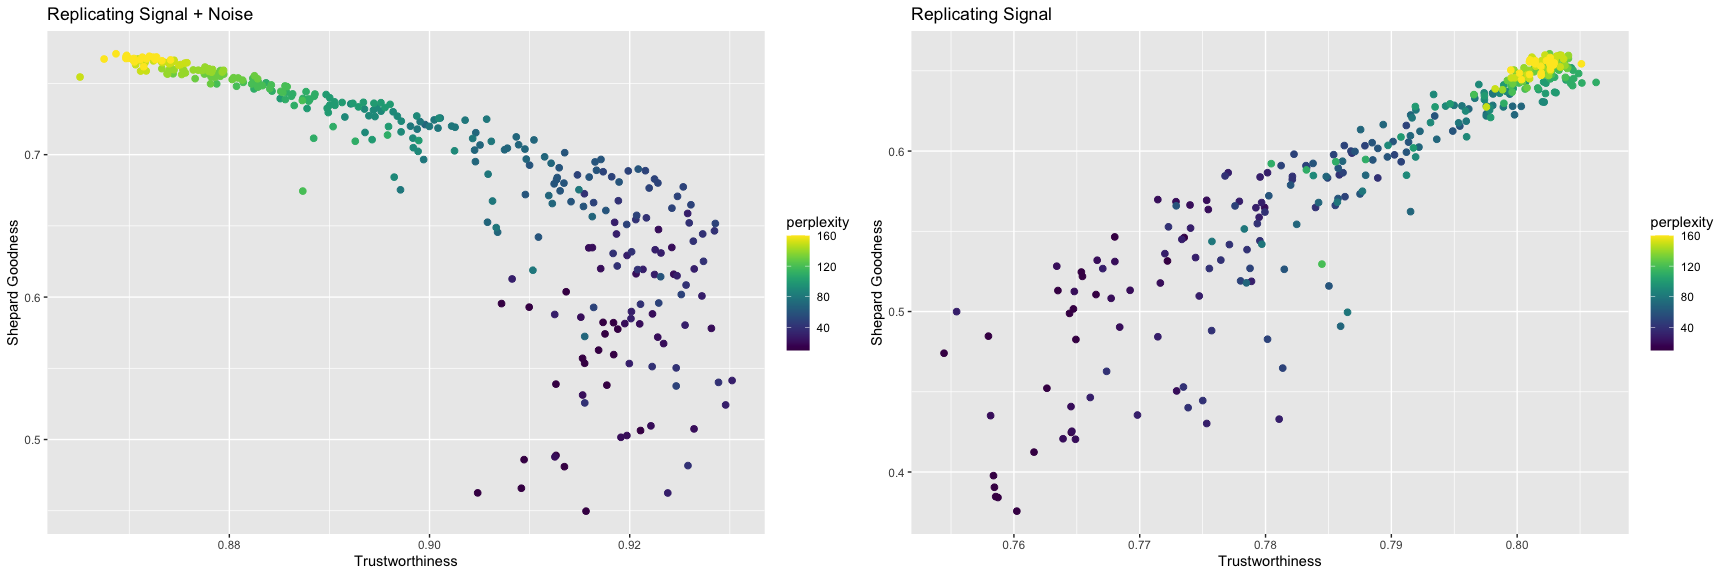
\includegraphics[scale=0.25]{trefoil plot}
\centering
\caption{Shepard Goodness vs. Trustworthiness (Trefoil Knot)}
\end{figure}

\begin{figure}[H]
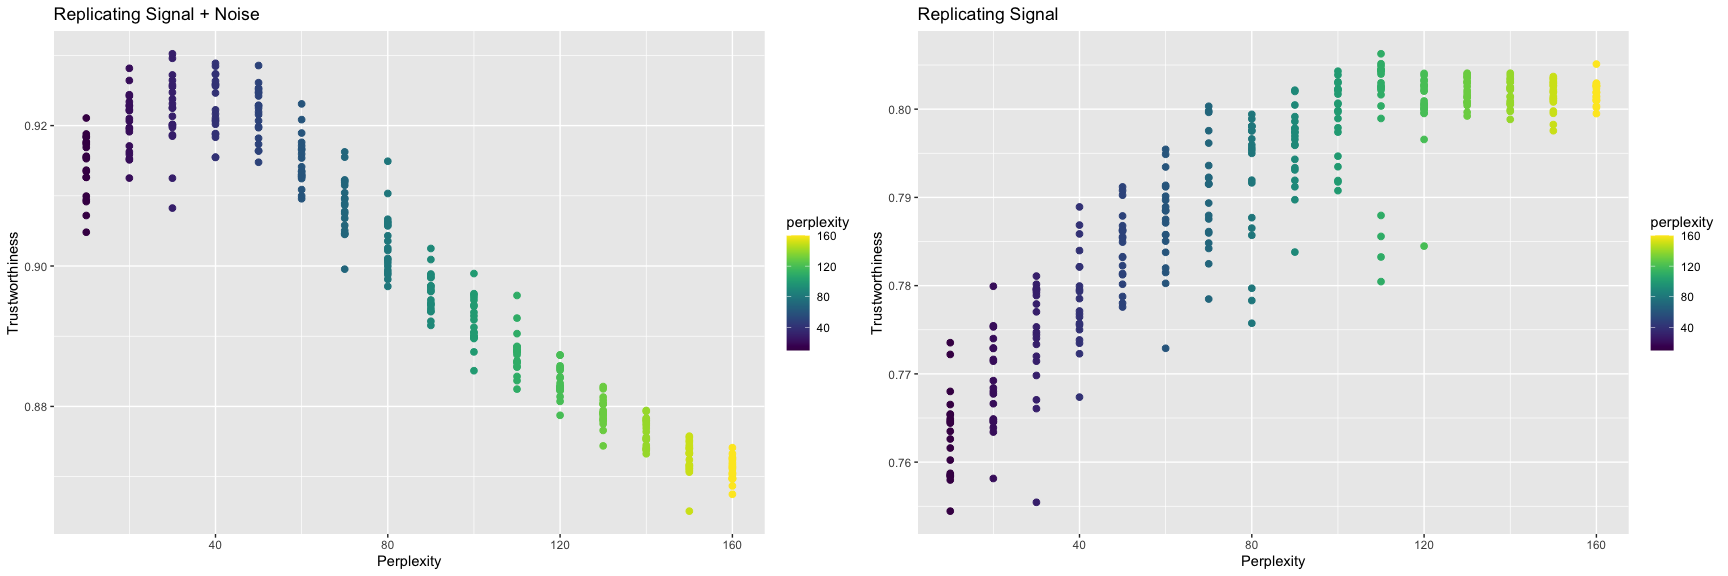
\includegraphics[scale=0.25]{trust plot (trefoil)}
\centering
\caption{Trustworthiness vs. Perplexity (Trefoil Knot)}
\end{figure}

\begin{figure}[H]
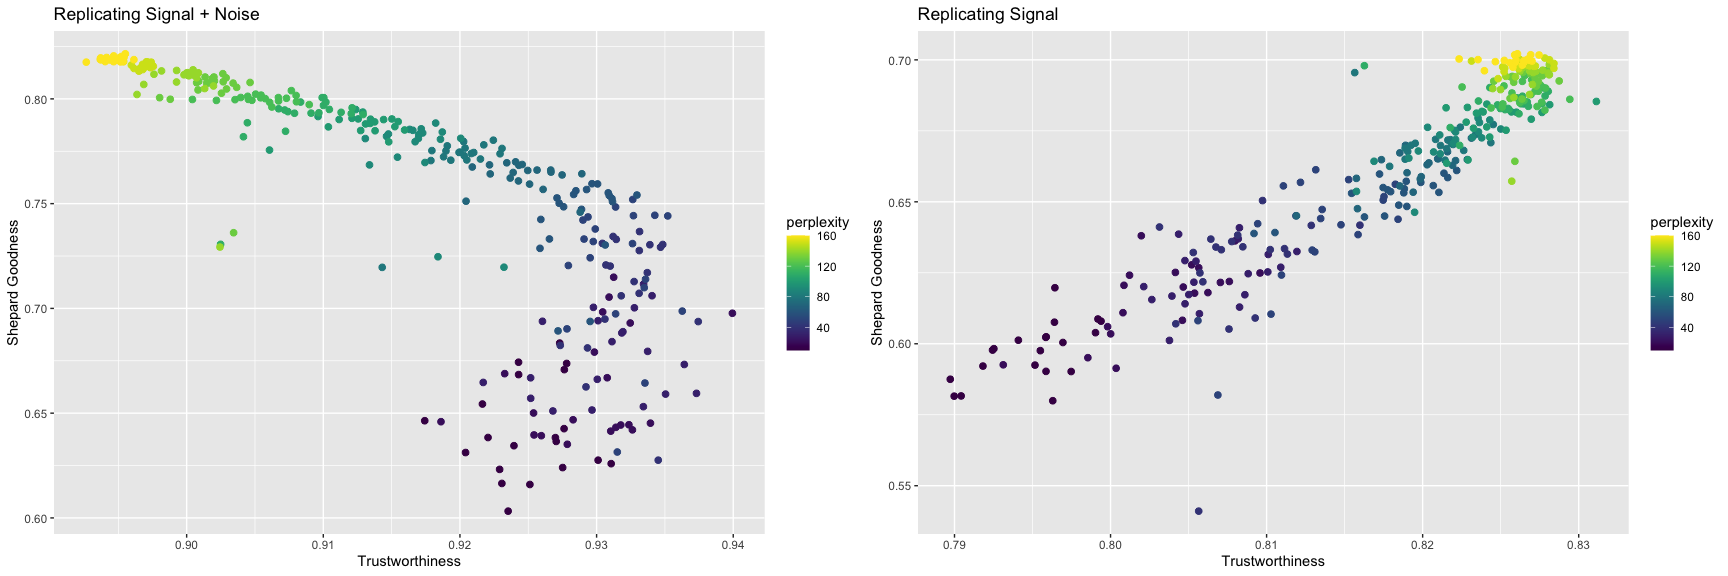
\includegraphics[scale=0.25]{mammoth plot}
\centering
\caption{Shepard Goodness vs. Trustworthiness (Mammoth)}
\end{figure}

\begin{figure}[H]
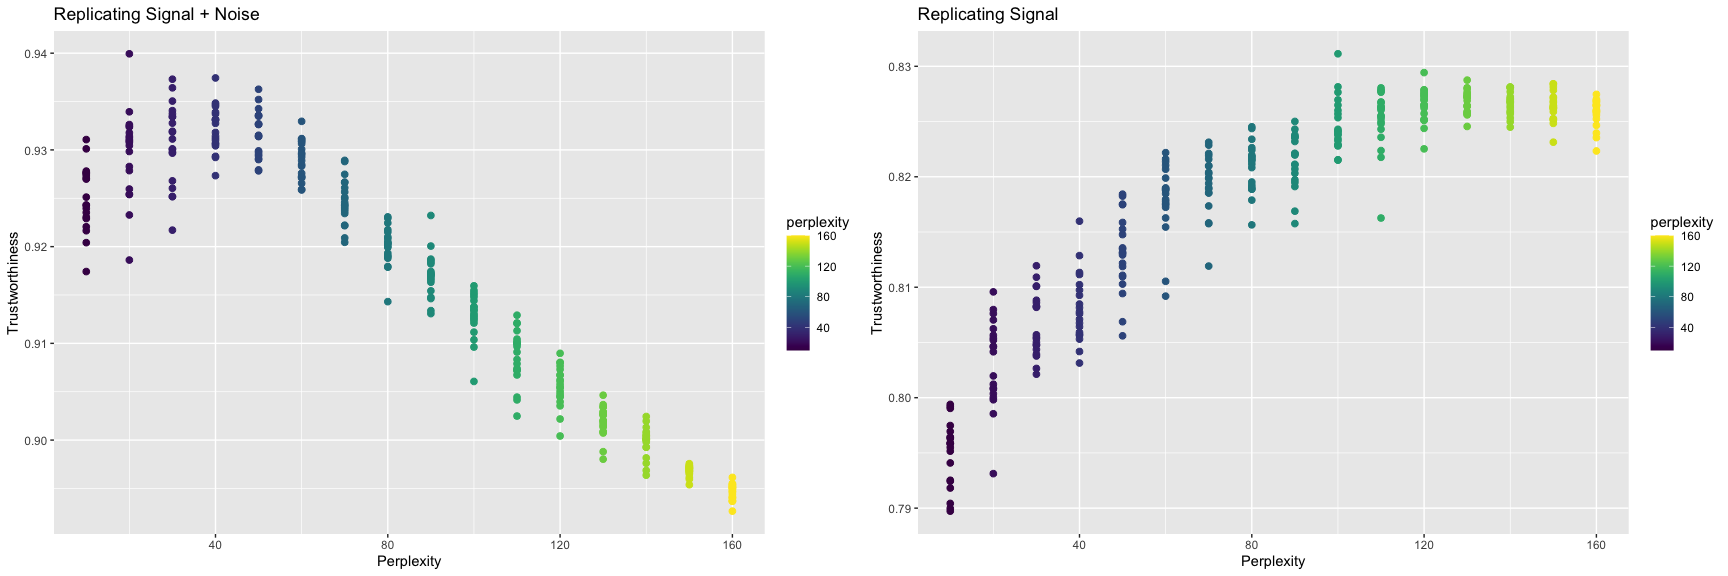
\includegraphics[scale=0.25]{trust plot (mammoth)}
\centering
\caption{Trustworthiness vs. Perplexity (Mammoth)}
\end{figure}

\subsection{Practical Examples}
For a practical example, we looked at a mass cytometry dataset containing 239,933 observations in 49 dimensions. To reduce the computational load, a subset of 5,000 observations were taken. Following the ordinary t-SNE workflow, a PCA pre-processing step was taken to reduce the number of dimensions to 10. A log transformation was also administered. The processed data set to be studied consisted of 5,000 observations in 10 dimensions, $$Z + \epsilon \in \mathbb{R}^{5,000 \times 10}.$$  $Y$ was extracted by taking the first two principal components, $$Y = \textrm{PCA}_2(Z + \epsilon).$$ We computed the t-SNE representations for perplexity values ranging from 20 to 1,600. For each perplexity value, 20 different t-SNE representations were computed. Below are the plots for $f_\textrm{Shep}(Z + \epsilon, X)$ vs. $f_\textrm{trust}(Z + \epsilon, X)$ and $f_\textrm{Shep}(Y, X)$ vs. $f_\textrm{trust}(Y, X)$:

\begin{figure}[H]
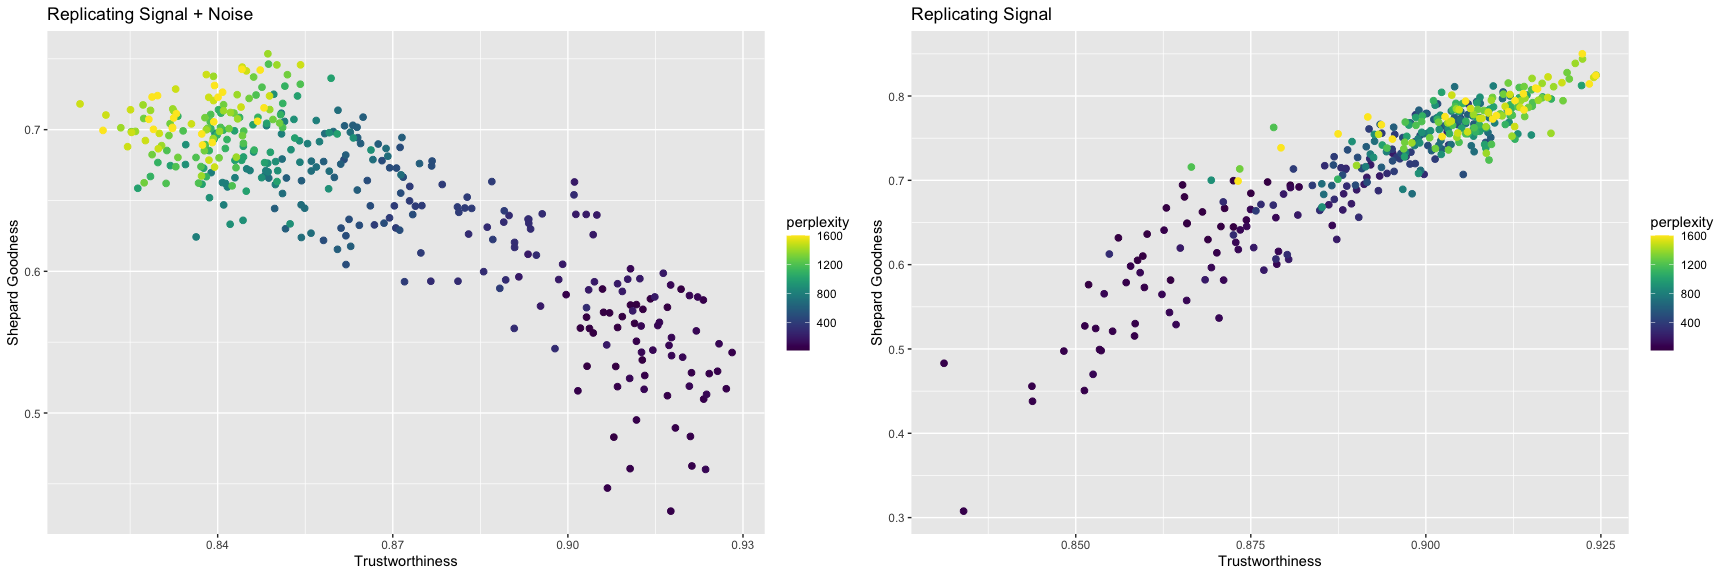
\includegraphics[scale=0.25]{CyTOF plot}
\centering
\caption{Shepard Goodness vs. Trustworthiness (CyTOF)}
\end{figure}

As with the generated examples, there is a difference in trend when comparing the low dimensional representation to the original data and just the underlying signal. More specifically, the t-SNE representations better locally represent the original data for lower perplexities and better locally represent the underlying signal for larger perplexities:

\begin{figure}[H]
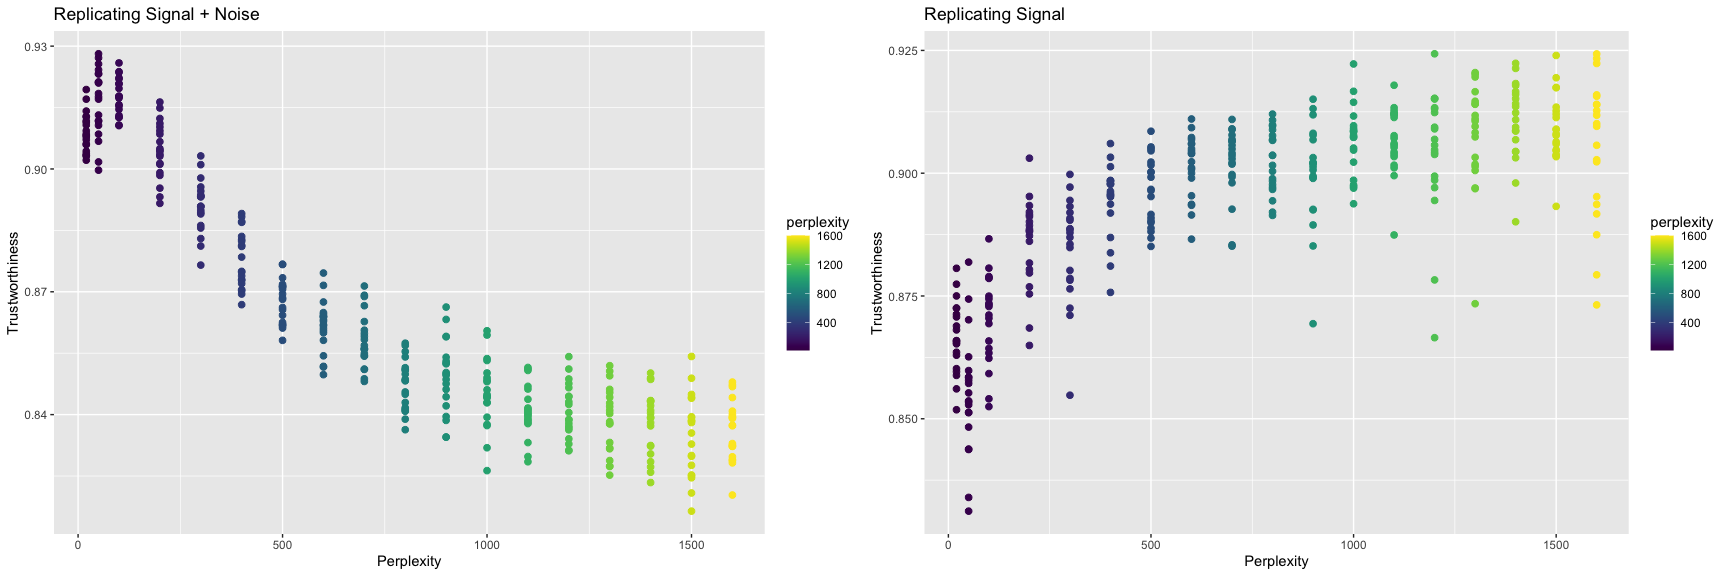
\includegraphics[scale=0.25]{trust plot (CyTOF)}
\centering
\caption{Trustworthiness vs. Perplexity (CyTOF)}
\end{figure}

When compared against the original data, trustworthiness is maximized when perplexity was set to 50, which is consistent with Kobak and Berens' recommendation of setting perplexity to $n/100$ \cite{t-SNE cell}. When compared against the underlying signal, trustworthiness is maximized at a much larger value of perplexity ($\sim 1,400$). These results are consistent with the hypothesis that lower values of perplexity may be overfitting the noise.

\bigbreak If we, instead, decide to be a little more conservative and use the first three principal components to represent the signal, we still see a similar trend.

\begin{figure}[H]
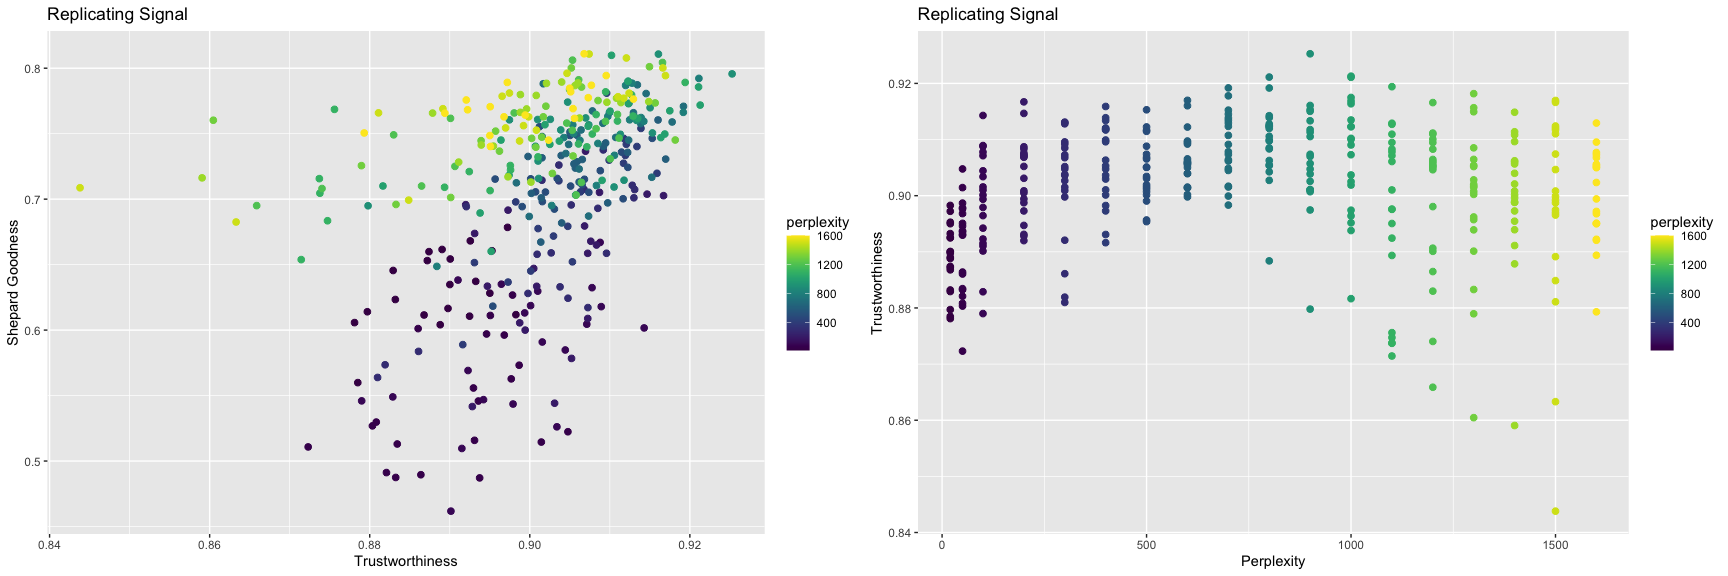
\includegraphics[scale=0.25]{3 dim plot (CyTOF)}
\centering
\caption{Shepard Goodness vs. Trustworthiness (CyTOF)}
\end{figure}

Trustworthiness still increases then decreases with perplexity. In this case, however, trustworthiness peaks at a perplexity around 900, less than before. By including an extra principal component in the signal, we're assuming the data contains less noise, so our model can be more aggressive during the fitting process. A lower perplexity corresponds to a more aggressive model with higher variance.

\section{Discussion}

\section{Application}
To apply this framework in practice, one must decide how to extract the signal from the data. The signal should include the features of the data one desires to retain throughout the dimension reduction process. When using a PCA projection to serve as the signal, one could draw a scree plot or employ component selection algorithms such as parallel analysis to determine the dimension of the signal. 

\bigbreak With a signal constructed, it remains to compute t-SNE outputs at varying perplexities. It's recommended that at least a couple of outputs are computed for each perplexity to account for t-SNE's inherit randomness. For each output, one must calculate the trustworthiness and Shepard goodness with respect to the signal. From there, one can choose the representation with the desirable balance of local and global performance.

\bigbreak It is worth noting that computational barriers may arise, especially for very large data sets. To alleviate such issues, trustworthiness and Shepard goodness can be approximated by subsampling before calculations. Furthermore, t-SNE is generally robust to small changes in perplexity \cite{t-SNE}, so checking a handful of different perplexities is sufficient. If computing the t-SNE representations is the limiting factor, the perplexity can be calibrated for a subsample of the data. \cite{subsample t-SNE} found that embedding a $\rho$-sample, where $\rho \in (0,1]$ is the sampling rate, with perplexity $\textrm{Perp}'$ gives a visual impression of embedding the original data with perplexity $$\textrm{\textrm{Perp}} = \frac{\textrm{Perp}'}{\rho}.$$ With these concessions, using this framework to calibrate perplexity is feasible for data sets of any size.

\section{Conclusion}

\newpage\begin{thebibliography}{10}

\bibitem{TriMap}
Amid and Warmuth. TriMap: Large-scale dimensionality reduction using triplets. arXiv:1910.00204v2 (2022).

\bibitem{perplexity vs kl}
Cao and Wang. Automatic selection of t-SNE perplexity. arXiv:1708.03229.v1 (2017).

\bibitem{large DR unreliable}
Chari and Pachter. The specious art of single-cell genomics. PLOS Computational Biology (2023). https://doi.org/10.1371/journal.pcbi.1011288

\bibitem{perplexity-free t-SNE}
Crecchi et al. Perplexity-free parametric t-SNE. arXiv:2010.01359v1 (2020).

\bibitem{quantitative survey}
Espadoto, et al. Towards a quantitative survey of dimension reduction techniques. IEEE Transactions on Visualization and Computer Graphics, Vol 27, No. 3 (2021).

\bibitem{t-SNE cell}
Kobak and Berens. The art of using t-SNE for single-cell transcriptomics. Nature Communications 10, 5416 (2019). https://doi.org/10.1038/s41467-019-13056-x

\bibitem{rank-based criteria}
Lee and Verleysen. Quality assessment of dimensionality reduction: Rank-based criteria. Neurocomputing 72, 1431 -- 1443 (2009).

\bibitem{precision score}
Schreck, et al. Techniques for precision-based visual analysis of projected data. Sage, Volume 9, Issue 3 (2012). https://doi.org/10.1057/ivs.2010.2

\bibitem{subsample t-SNE}
Skrodzki, et al. Tuning the perplexity for and computing sampling-based t-SNE embeddings. arXiv:2308.15513v1 (2023).
 
\bibitem{t-SNE}
van der Maaten and Hinton. Visualizing data using t-SNE. Journal of Machine Learning Research 9, 2579 -- 2605 (2008).

\bibitem{trustworthiness}
Venna and Kaski. Visualizing gene interaction graphs with local multidimensional scaling. European Symposium on Artificial Neural Networks (2006).

\bibitem{understanding DR}
Wang, et al. Understanding how dimension reduction tools work: An empirical approach to deciphering t-SNE, UMAP, TriMap, and PaCMAP for data visualization. Journal of Machine Learning Research 22 (2021).

\bibitem{Distill}
Wattenberg, et al. How to Use t-SNE Effectively. Distill (2016). http://doi.org/10.23915/distil

\end{thebibliography}

\end{document}